\documentclass[12pt]{article}
\usepackage[a4paper, inner=1.5cm, outer=3cm, top=2cm,bottom=3cm, bindingoffset=1cm]{geometry}
\usepackage[english]{babel}
\usepackage[utf8x]{inputenc}
\usepackage{import}
\usepackage{amsmath}
\usepackage{tikz}
\usepackage[maxfloats=256]{morefloats}
\usepackage{booktabs}
\usepackage{graphicx}
\usepackage{hyperref}
\usepackage{pdflscape}
\usepackage{adjustbox}
\graphicspath{ {./images/} }
\usepackage{capt-of} 
\usepackage{listings}
\usepackage{xcolor}
\usepackage{setspace}
\definecolor{codegreen}{rgb}{0,0.6,0}
\definecolor{codegray}{rgb}{0.5,0.5,0.5}
\definecolor{codepurple}{rgb}{0.58,0,0.82}
\definecolor{backcolour}{rgb}{0.95,0.95,0.92}
\maxdeadcycles=1000

\lstdefinestyle{mystyle}{
    backgroundcolor=\color{backcolour},   
    commentstyle=\color{codegreen},
    keywordstyle=\color{magenta},
    numberstyle=\tiny\color{codegray},
    stringstyle=\color{codepurple},
    basicstyle=\ttfamily\footnotesize,
    breakatwhitespace=false,         
    breaklines=true,                 
    captionpos=b,                    
    keepspaces=true,                 
    numbers=left,                    
    numbersep=5pt,                  
    showspaces=false,                
    showstringspaces=false,
    showtabs=false,                  
    tabsize=2
}
 
\lstset{style=mystyle}

\begin{document}
\begin{titlepage}
\newcommand{\HRule}{\rule{\linewidth}{0.5mm}} 
\center
\doublespacing
\textbf{\Huge MACHINE LEARNING FOR PREDICTING DIABETES MELLITUS}
\\
\singlespacing
\Large
\vspace{3cm}
A project report submitted in partial fulfilment of the requirement for the degree of\\
\vspace{1cm}
\textbf{Bachelor in Science\\In\\Computer Science}
\\by\\
\Large
Alexander Roque Rodrigues
\\
\vspace{1cm}
under the supervision of
\vspace{1cm}
\\
Ashweta Fondekar
\\
\textbf{PARVATIBAI CHOWGULE COLLEGE OF ARTS \& SCIENCE AUTONOMOUS}
\\June 2019
\end{titlepage}

%declaration
\onehalfspacing
%\doublespacing
\newpage
\vspace{15cm}
\begin{center}

\Huge{\textbf{Declaration by Candidate}}\\
\normalsize
I declare that this project report has been prepared by me and to the best of my
knowledge, it has not previously formed the basis for the award of any diploma or degree by
any other University.
\end{center}
\newpage
\vspace{15cm}

\begin{center}
\Huge{\textbf{Certificate by Supervisor}}\\
\normalsize
Certified that the Project Report is a record of work done by the candidate himself/herself/themselves under my guidance during the period of study and that to the best of my knowledge, it has not previously formed the basis of the award of any degree or diploma of any other University.\\
\vspace{5cm}
Ashweta Fondekar\\

Project Supervisor
\end{center}
\newpage

\textbf{Work Record}


\newpage
\section{Acknowledgements}

\newpage
\tableofcontents
\newpage
\listoffigures
\newpage
\listoftables
\newpage


\begin{abstract}
Diabetes Mellitus is a disease that prevents the body from properly expanding the
energy stored from the food consumed. The purpose of this project was to select
machine learning algorithms that are able to predict or classify a person as diabetic
or healthy based on the legacy data. The algorithms compared were KNN
Classifier, Logistic Regression, Decision Tree Classifier, Random Forest
Classifier, Gradient Boosting Classifier, Support Vector Classifier and the
Multi-Layered Perceptron. From all the above the Multi-Layered Perceptron gave
an accuracy of prediction on the dataset as ~79.70\%. To improve the performance
of the classifier, I have considered new features deduced from the currently
existing feature set a re-trained the classifier on the new dataset that I generated,
which is now able to classify the subject as diabetic or healthy with a new accuracy
of ~93.10\%. A significant change which boosted the accuracy by 13.4\%. After
selection of the algorithm I further advanced the platform of cluster computing to
deploy the algorithm onto and generate predictions in without any human
interference (apart from entering the data itself) ​ and also made the data available
to the users via an easy to use web application which gives them access to the
observations then stored in the database after being predicted by the algorithm
deployed on the nodes.
\end{abstract}


\section{Introduction}
In recent days, there has been a sharp increase in the cases of diabetes mellitus. Diabetes mellitus is on the rise amongst many people and the rate of contracting this lifestyle disease could be reduced significantly if proper measures and precautions were to be instilled amongst people the number of people can be reduced.

Machine learning is a growing field in computer science. With the development and introduction of many algorithms the prediction and accuracy of the predictions itself has improved substantially. Machine learning and healthcare systems are also becoming increasingly popular in the healthcare sector.

The project encompasses the qualities of Remote Patient Monitoring (RPM) and Clinical Decision Support (CDS). RPM provides medical facilities that have the ability to transmit patient data to healthcare professionals who might very well be halfway around the world. RPM can monitor blood glucose levels and blood pressure. It is particularly helpful for patients with chronic conditions such as type 2 diabetes, hypertension, or cardiac disease. Data collected and transmitted via PRM can be used by a healthcare professional or a healthcare team to detect medical events such as stroke or heart attack that require immediate and aggressive medical intervention. Data collected may be used as part of a research project or health study. RPM is a life-saving system for patients in remote areas who cannot access face-to-face health care. CDS analyzes data from clinical and administrative systems. The aim is to assist healthcare providers in making informed clinical decisions. Data available can provide information to medical professions who are preparing diagnoses or predicting medical conditions like drug interactions and reactions. CDS tools filter information to assist healthcare professionals in caring for individual clients. 

The objective of this project is to create a  system that is able to use the machine learning algorithms and predict the outcome of the parameters entered into the algorithm and help the patient draw a conclusion whether or not he/she has the same traits exhibited by similar patients that have diabetes. Also the system should have a UI that is capable of displaying the data of the patients to the doctor and to the patients themselves for further interpretation.

\newpage
\section{Project Rationale}
Key facts
The number of people with diabetes has risen from 108 million in 1980 to 422 million in 2014.
The global prevalence of diabetes* among adults over 18 years of age has risen from 4.7\% in 1980 to 8.5\% in 2014 (1).
Diabetes prevalence has been rising more rapidly in middle- and low-income countries.
Diabetes is a major cause of blindness, kidney failure, heart attacks, stroke and lower limb amputation.
In 2016, an estimated 1.6 million deaths were directly caused by diabetes. Another 2.2 million deaths were attributable to high blood glucose in 2012**.
Almost half of all deaths attributable to high blood glucose occur before the age of 70 years. WHO estimates that diabetes was the seventh leading cause of death in 2016.
Healthy diet, regular physical activity, maintaining a normal body weight and avoiding tobacco use are ways to prevent or delay the onset of type 2 diabetes.
Diabetes can be treated and its consequences avoided or delayed with diet, physical activity, medication and regular screening and treatment for complications.
What is diabetes?
Diabetes is a chronic disease that occurs either when the pancreas does not produce enough insulin or when the body cannot effectively use the insulin it produces. Insulin is a hormone that regulates blood sugar. Hyperglycaemia, or raised blood sugar, is a common effect of uncontrolled diabetes and over time leads to serious damage to many of the body's systems, especially the nerves and blood vessels.

In 2014, 8.5\% of adults aged 18 years and older had diabetes. In 2016, diabetes was the direct cause of 1.6 million deaths and in 2012 high blood glucose was the cause of another 2.2 million deaths.

Type 1 diabetes
Type 1 diabetes (previously known as insulin-dependent, juvenile or childhood-onset) is characterized by deficient insulin production and requires daily administration of insulin. The cause of type 1 diabetes is not known and it is not preventable with current knowledge.

Symptoms include excessive excretion of urine (polyuria), thirst (polydipsia), constant hunger, weight loss, vision changes, and fatigue. These symptoms may occur suddenly.

Type 2 diabetes
Type 2 diabetes (formerly called non-insulin-dependent, or adult-onset) results from the body’s ineffective use of insulin. Type 2 diabetes comprises the majority of people with diabetes around the world, and is largely the result of excess body weight and physical inactivity.

Symptoms may be similar to those of type 1 diabetes, but are often less marked. As a result, the disease may be diagnosed several years after onset, once complications have already arisen.

Until recently, this type of diabetes was seen only in adults but it is now also occurring increasingly frequently in children.

Gestational diabetes
Gestational diabetes is hyperglycaemia with blood glucose values above normal but below those diagnostic of diabetes, occurring during pregnancy.

Women with gestational diabetes are at an increased risk of complications during pregnancy and at delivery. They and their children are also at increased risk of type 2 diabetes in the future.

Gestational diabetes is diagnosed through prenatal screening, rather than through reported symptoms.

Impaired glucose tolerance and impaired fasting glycaemia
Impaired glucose tolerance (IGT) and impaired fasting glycaemia (IFG) are intermediate conditions in the transition between normality and diabetes. People with IGT or IFG are at high risk of progressing to type 2 diabetes, although this is not inevitable.

What are common consequences of diabetes?
Over time, diabetes can damage the heart, blood vessels, eyes, kidneys, and nerves.

Adults with diabetes have a two- to three-fold increased risk of heart attacks and strokes (1).
Combined with reduced blood flow, neuropathy (nerve damage) in the feet increases the chance of foot ulcers, infection and eventual need for limb amputation.
Diabetic retinopathy is an important cause of blindness, and occurs as a result of long-term accumulated damage to the small blood vessels in the retina. 2.6\% of global blindness can be attributed to diabetes (2).
Diabetes is among the leading causes of kidney failure (3).
How can the burden of diabetes be reduced?
Prevention
Simple lifestyle measures have been shown to be effective in preventing or delaying the onset of type 2 diabetes. To help prevent type 2 diabetes and its complications, people should:

achieve and maintain healthy body weight;
be physically active – at least 30 minutes of regular, moderate-intensity activity on most days. More activity is required for weight control;
eat a healthy diet, avoiding sugar and saturated fats intake; and
avoid tobacco use – smoking increases the risk of diabetes and cardiovascular diseases.
Diagnosis and treatment
Early diagnosis can be accomplished through relatively inexpensive testing of blood sugar.

Treatment of diabetes involves diet and physical activity along with lowering blood glucose and the levels of other known risk factors that damage blood vessels. Tobacco use cessation is also important to avoid complications.

Interventions that are both cost-saving and feasible in developing countries include:

blood glucose control, particularly in type 1 diabetes. People with type 1 diabetes require insulin, people with type 2 diabetes can be treated with oral medication, but may also require insulin;
blood pressure control; and
foot care.
Other cost saving interventions include:

screening and treatment for retinopathy (which causes blindness)
blood lipid control (to regulate cholesterol levels)
screening for early signs of diabetes-related kidney disease and treatment.

\newpage
\section{Software Requirements}
The main function of this project is to enable the doctors to advise their patients with the help of the prediction software. The system should be accessible to the patient as well as the doctor, therefore it should have a web interface for the two parties to interact with.

\subsection{Functionalities for Doctors}
As an owner of a doctors account a doctor should be able to:
\begin{itemize}
\item Add new observations for the machine learning algorithm to predict.
\item Analyse the patients previous records.
\item Have a dashboard for patient performance monitoring.
\end{itemize}

\subsection{Functionalities for Patients}
As the patient, one should be able to:
\begin{itemize}
\item Should be able to see the predicted risk of developing diabetes.
\item Should be able to view historic data.
\end{itemize}

\subsection{Functionalities for Master Nodes}
As the master nodes:
\begin{itemize}
\item Control chunk size.
\item Remotely update the slave nodes.
\item Check the status of nodes.
\item Control the SQL database.
\end{itemize}

\subsection{Functionalities for Slave Nodes}
\begin{itemize}
\item Should have the machine learning algorithm tuned as per specifications.
\item Remote update should be possible.
\item Remote access should be possible.
\end{itemize}

\newpage
\section{Hardware Requirements}
\subsection{Raspberry Pi}

According to raspberrypi.org, the Raspberry Pi 3 Model B is the earliest model of the third-generation Raspberry Pi. It replaced the Raspberry Pi 2 Model B in February 2016. Some of the key features of this single board computer or SBC are:
\begin{itemize}
\item Quad Core 1.2GHz Broadcom BCM2837 64bit CPU.
\item 1GB RAM.
\item BCM43438 wireless LAN and Bluetooth Low Energy (BLE) on board.
\item 100 Base Ethernet.
\item 40-pin extended GPIO.
\item 4 USB 2 ports.
\item Full size HDMI.
\item Micro SD port for loading the operating system and storing data.
\end{itemize}
In this project I will be using 3 Raspberry Pi's to implement a cluster and deploy the machine learning algorithm on.

\subsection{Switch}
A network switch was used in the project to make up for the lack of ethernet ports available on the router.

\subsection{Router}
A router is required to assign internet protocol addresses to the nodes using dynamic host control protocol (DHCP). The router also is responsible for displaying the nodes connected to the network thereby displaying host names and making it more easier to capture the addresses of each node.

\subsection{Master Node}
The master node is assigned the task of managing the the slave nodes connected to the network. The master node and the slave nodes should be connected to the same database to run and execute queries. The master node shall also be assigned with the task of killing a particular process or shutting down a particular node if required.

\subsection{Slave Node}
The slave nodes are to be configured with the selected algorithm and are the most vital part of the structure. The slave nodes will be responsible for receiving instructions from the master node and will be responsible for learning from the dataset and then can generate predicted outcomes for the patient records received from the master. 

\subsection{Database}
The database will store all the records for the patients and doctors. The database is a SQL database that will not be subjected to a change in the database schema structure for consistency.

\subsection{Web Server}
The web server provides an interface for the doctor and the patients to read the predictions and legacy data of the patient from the website.

\newpage
\section{Technology Stack}
\subsection{Python}
\subsubsection{Pandas}
Pandas, is a library that is required for loading the comma separated value file into python. Pandas is a package for data manipulation and analysis. In particular, it offers data structures and operations for manipulating numerical tables and time series.

\subsubsection{Sklearn}
Scikit-learn is a free software machine learning library for the Python programming language. It features various classification, regression and clustering algorithms including support vector machines, random forests, gradient boosting, k-means and DBSCAN, and is designed to inter-operate with the Python numerical and scientific libraries NumPy and SciPy.

\subsubsection{Numpy}
NumPy is a library for the Python programming language, adding support for large, multi-dimensional arrays and matrices, along with a large collection of high-level mathematical functions to operate on these arrays. NumPy is open-source software and has many contributors.

\subsubsection{Itertools}
The itertools module standardizes a core set of fast, memory efficient tools that are useful by themselves or in combination. Together, they form an “iterator algebra” making it possible to construct specialized tools succinctly and efficiently in pure Python.

\subsection{MYSQL}
MySQL is an open-source relational database management system. MySQL is free and open-source software under the terms of the GNU General Public License, and is also available under a variety of proprietary licenses. MySQL was owned and sponsored by the Swedish company MySQL AB, which was bought by Sun Microsystems (now Oracle Corporation). MySQL is a component of the LAMP web application software stack (and others), which is an acronym for Linux, Apache, MySQL, Perl/PHP/Python. MySQL is used by many database-driven web applications, including Drupal, Joomla, phpBB, and WordPress. MySQL is also used by many popular websites, including Facebook, Flickr, MediaWiki, Twitter and YouTube.

\subsection{Apache Web Server}
The Apache HTTP Server, colloquially called Apache, is free and open-source cross-platform web server software, released under the terms of Apache License 2.0. Apache is developed and maintained by an open community of developers under the auspices of the Apache Software Foundation. The vast majority of Apache HTTP Server instances run on a Linux distribution, but current versions also run on Microsoft Windows and a wide variety of Unix-like systems. Past versions also ran on OpenVMS, NetWare, OS/2 and other operating systems, including ports to mainframes.

\subsection{PHP}
PHP is a general-purpose programming language originally designed for web development. PHP originally stood for Personal Home Page,
but it now stands for the recursive initialism PHP: Hypertext Preprocessor. PHP code may be executed with a command line interface (CLI), embedded into HTML code, or used in combination with various web template systems, web content management systems, and web frameworks. PHP code is usually processed by a PHP interpreter implemented as a module in a web server or as a Common Gateway Interface (CGI) executable. The web server outputs the results of the interpreted and executed PHP code, which may be any type of data, such as generated HTML code or binary image data. PHP can be used for many programming tasks outside of the web context, such as standalone graphical applications and robotic drone control.

\subsection{AJAX}
Ajax is a set of web development techniques using many web technologies on the client side to create asynchronous web applications. With Ajax, web applications can send and retrieve data from a server asynchronously (in the background) without interfering with the display and behavior of the existing page. By decoupling the data interchange layer from the presentation layer, Ajax allows web pages and, by extension, web applications, to change content dynamically without the need to reload the entire page.[3] In practice, modern implementations commonly utilize JSON instead of XML.

Ajax is not a single technology, but rather a group of technologies. HTML and CSS can be used in combination to mark up and style information. The webpage can then be modified by JavaScript to dynamically display—and allow the user to interact with—the new information. The built-in XMLHttpRequest object, or since 2017 the new "fetch()" function within JavaScript, is commonly used to execute Ajax on web pages allowing websites to load content onto the screen without refreshing the page. Ajax is not a new technology, or different language, just existing technologies used in new ways.

\subsection{GitHub}
GitHub is a global company that provides hosting for software development version control using Git. It offers all of the distributed version control and source code management (SCM) functionality of Git as well as adding its own features. It provides access control and several collaboration features such as bug tracking, feature requests, task management, and wikis for every project.

\subsection{SSH}
Secure Shell is a cryptography network protocol for operating network services securely over an unsecured network. Typical applications include remote command-line, login, and remote command execution, but any network service can be secured with SSH. The SSH is used to communicate between the master and slave nodes.

\newpage
\section{Methodology}
The dataset used for this project is from the UCI Machine learning repository and can be found at their respective website. Table \ref{table:2} is an outcome of the accuracy of the algorithms subjected to train and \ref{table:3} is the accuracy obtained from the predicted outcomes for given sets of patients.

Firstly, I began the experiment by examining the amount of people that were recorded by the dataset. We can see that the dataset contains a total of 768 observations. From figure \ref{fig:1} we can see that 268 people are healthy, while the rest of the 500 subjects are diabetic. If converted to percentage, 65.1\% of the subjects are healthy and 34.9\% of subjects are diabetic.

To proceed with the eploratory data analysis, we can examine the missing values in the dataset. 


\newpage
\section{Deploying to Cluster}
A cluster is a group of two or more servers connected to each other in such a way that they behave like a single server. Each machine in the cluster is called a node. Because each machine in the cluster runs the same services as other machines in the cluster, any machine can stand in for any other machine in the cluster. This becomes important when one machine goes down or must be taken out of service for a time. The remaining machines in the cluster can seamlessly take over the work of the downed machine, providing users with uninterrupted access to services and data.

\subsection{Benefits of Clustering}
\begin{itemize}
\item \texttt{Increased resource availability} If one Intelligence Server in a cluster fails, the other Intelligence Servers in the cluster can pick up the workload. This prevents the loss of valuable time and information if a server fails.
Strategic resource usage: You can distribute projects across nodes in whatever configuration you prefer. This reduces overhead because not all machines need to be running all projects, and allows you to use your resources flexibly.

\item \texttt{Increased performance} Multiple machines provide greater processing power.
\item \texttt{Greater scalability} As your user base grows and report complexity increases, your resources can grow.
\item \texttt{Simplified management} Clustering simplifies the management of large or rapidly growing systems.

Fail-over support ensures that a business intelligence system remains available for use if an application or hardware failure occurs. Clustering provides failover support in two ways:
\item
\texttt{Load redistribution} When a node fails, the work for which it is responsible is directed to another node or set of nodes.
Request recovery: When a node fails, the system attempts to reconnect MicroStrategy Web users with queued or processing requests to another node. Users must log in again to be authenticated on the new node. The user is prompted to resubmit job requests.

\item \texttt{Load Balancing}
Load balancing is a strategy aimed at achieving even distribution of user sessions across Intelligence Servers, so that no single machine is overwhelmed. This strategy is especially valuable when it is difficult to predict the number of requests a server will receive. MicroStrategy achieves four-tier load balancing by incorporating load balancers into the MicroStrategy Web and Web products. Load is calculated as the number of user sessions connected to a node. The load balancers collect information on the number of user sessions each node is carrying. Using this information at the time a user logs in to a project, MicroStrategy Web connects them to the Intelligence Server node that is carrying the lightest session load. All requests by that user are routed to the node to which they are connected until the user disconnects from the MicroStrategy Web product.

\item
\texttt{Project Distribution and Project Fail over}
When you set up several server machines in a cluster, you can distribute projects across those clustered machines or nodes in any configuration, in both Windows and Linux environments. All servers in a cluster do not need to be running all projects. Each node in the cluster can host a different set of projects, which means only a subset of projects need to be loaded on a specific Intelligence Server machine. This feature provides you with flexibility in using your resources, and it provides better scalability and performance because of less overhead on each Intelligence Server machine. Distributing projects across nodes also provides project fail-over support. For example, one server is hosting project A and another server is hosting projects B and C. If the first server fails, the other server can host all three projects to ensure project availability. Project creation, duplication, and deletion in a three-tier, or server, connection are automatically broadcast to all nodes during run-time to ensure synchronization across the cluster.
\item
\texttt{Work Fencing}
User fences and workload fences allow you to reserve nodes of a cluster for either users or a project subscriptions. 

\end{itemize}

\newpage
\section{Future Scope}

\newpage

{
\clearpage
\thispagestyle{empty}
\begin{landscape}
\centering
\begin{table}[]
\centering
\section{Tables}
\begin{tabular}{|l|l|}
\hline
Column Name                & Description                                                               \\ \hline
Pregnancies                & Number of times pregnant.                                                 \\ \hline
Glucose                    & Plasma glucose concentration a 2 hours in an oral glucose tolerance test. \\ \hline
Blood Pressure             & Diastolic blood pressure (mm Hg)                                          \\ \hline
Skin Thickness             & Triceps skin fold thickness (mm)                                          \\ \hline
Insulin                    & 2-Hour serum insulin (muU/ml)                                            \\ \hline
Body Mass Index            & Body mass index (weight in kg/(height in m)\textasciicircum{}2)           \\ \hline
Diabetes Pedigree Function & Diabetes pedigree function                                                \\ \hline
Age                        & Age (years)                                                               \\ \hline
Outcome                    & Class variable (0 or 1) 268 of 768 are 1, the others are 0                \\ \hline
\end{tabular}
\end{table}
\captionof{table}{Pima Indians dataset header.}
\label{table:1}
\end{landscape}
\clearpage
}


{
\clearpage
\thispagestyle{empty}
\begin{landscape}
\centering
\begin{table}[]
\centering
\begin{tabular}{|c|c|c|c|}
\hline
Algorithm              & Additional Parameters                              & Train Set Accuracy \\ \hline
K Nearest Neighbour    & -                                                  & 0.790               \\ \hline
Logistic Regression    & C = 1                                              & 0.781              \\ \hline
Logistic Regression    & C = 0.01                                           & 0.700              \\\hline
Logistic Regression    & C = 100                                            & 0.785              \\ \hline
Decision Tree          & -                                                  & 1.000              \\ \hline
Decision Tree          & Max Depth = 3                                      & 0.773              \\ \hline
Random Forest          & Estimators = 100                                   & 1.000              \\ \hline
Random Forest          & Estimators = 100; Max Depth = 3                    & 0.800              \\ \hline
Gradient Boosting      & -                                                  & 0.917              \\ \hline
Gradient Boosting      & Max Depth = 1                                      & 0.804              \\ \hline
Gradient Boosting      & Learning Rate = 0.01                               & 0.802              \\ \hline
Support Vector Machine & -                                                  & 1.000              \\ \hline
Support Vector Machine & Train and Test set scaled using MinMaxScaler       & 0.770              \\ \hline
Support Vector Machine & C = 1000                                           & 0.790              \\ \hline
MLP Classifier         & Random State = 42                                  & 0.730              \\ \hline
MLP Classifier         & Random State = 0                                   & 0.823              \\ \hline
MLP Classifier         & Max Iterations = 1000                              & 0.908              \\ \hline
MLP Classifier         & Max Iterations = 1000; Alpha = 1; Random State = 0 & 0.806              \\ \hline
\end{tabular}
\end{table}
\captionof{table}{Train accuracy using various machine learning algorithms with various parameters.}
\label{table:2}
\end{landscape}
\clearpage
}


{
\clearpage
\thispagestyle{empty}
\begin{landscape}
\centering
\begin{table}[]
\centering
\begin{tabular}{|c|c|c|c|}
\hline
Algorithm              & Additional Parameters                               & Test Set Accuracy \\ \hline
K Nearest Neighbour    & -                                                   & 0.780             \\ \hline
Logistic Regression    & C = 1                                               & 0.771             \\ \hline
Logistic Regression    & C = 0.01                                            & 0.703             \\ \hline
Logistic Regression    & C = 100                                             & 0.766             \\ \hline
Decision Tree          & -                                                   & 0.714             \\ \hline
Decision Tree          & Max Depth = 3                                       & 0.740             \\ \hline
Random Forest          & Estimators = 100                                    & 0.786             \\ \hline
Random Forest          & Estimators = 100; Max Depth = 3                     & 0.755             \\ \hline
Gradient Boosting      & -                                                   & 0.792             \\ \hline
Gradient Boosting      & Max Depth = 1                                       & 0.781             \\ \hline
Gradient Boosting      & Learning Rate = 0.01                                & 0.776             \\ \hline
Support Vector Machine & -                                                   & 0.650             \\ \hline
Support Vector Machine & Train and Test set scaled using MinMaxScaler        & 0.770              \\ \hline
Support Vector Machine & C = 1000                                            & 0.797             \\ \hline
MLP Classifier         & Random State = 42                                   & 0.720              \\ \hline
MLP Classifier         & Random State = 0                                    & 0.802             \\ \hline
MLP Classifier         & Max Iterations = 1000                               & 0.792             \\ \hline
MLP Classifier         & Max Iterations = 1000; Alpha = 1; Random State = 0  & 0.797             \\ \hline
\end{tabular}
\end{table}
\captionof{table}{Test accuracy using various machine learning algorithms with various parameters.}
\label{table:3}
\end{landscape}
\clearpage
}

{
\clearpage
\thispagestyle{empty}
\centering
\begin{table}[]
\centering
\begin{tabular}{|l|l|l|}
\hline
Column                     & Number of Non-Zero Values & Percentage \\ \hline
Pregnancies                & 0                         & 0          \\ \hline
Glucose                    & 763                       & 0.65       \\ \hline
Blood Pressure             & 733                       & 4.56       \\ \hline
Skin Thickness             & 541                       & 29.56      \\ \hline
Insulin                    & 394                       & 48.7       \\ \hline
Body Mass Index            & 757                       & 1.43       \\ \hline
Diabetes Pedigree Function & 0                         & 0          \\ \hline
Age                        & 0                         & 0          \\ \hline
Outcome                    & 0                         & 0          \\ \hline
\end{tabular}
\end{table}
\captionof{table}{Null Value Check.}
\label{table:4}
\clearpage
}

\newpage
\section{Appendix I}
\subsection{K Nearest Neighbours}
\begin{lstlisting}
class sklearn.neighbors.KNeighborsClassifier(n_neighbors=5, weights='uniform', algorithm='auto', leaf_size=30, p=2, metric='minkowski', metric_params=None, n_jobs=None, **kwargs)
\end{lstlisting}

\subsection{Logistic Regression}
\begin{lstlisting}
class sklearn.linear_model.LogisticRegression(penalty='l2', dual=False, tol=0.0001, C=1.0, fit_intercept=True, intercept_scaling=1, class_weight=None, random_state=None, solver='lbfgs', max_iter=100, multi_class='auto', verbose=0, warm_start=False, n_jobs=None, l1_ratio=None)
\end{lstlisting}

\subsection{Decision Tree}
\begin{lstlisting}
class sklearn.tree.DecisionTreeClassifier(criterion='gini', splitter='best', max_depth=None, min_samples_split=2, min_samples_leaf=1, min_weight_fraction_leaf=0.0, max_features=None, random_state=None, max_leaf_nodes=None, min_impurity_decrease=0.0, min_impurity_split=None, class_weight=None, presort='deprecated', ccp_alpha=0.0)
\end{lstlisting}

\subsection{Random Forest Classifier}
\begin{lstlisting}
class sklearn.ensemble.RandomForestClassifier(n_estimators=100, criterion='gini', max_depth=None, min_samples_split=2, min_samples_leaf=1, min_weight_fraction_leaf=0.0, max_features='auto', max_leaf_nodes=None, min_impurity_decrease=0.0, min_impurity_split=None, bootstrap=True, oob_score=False, n_jobs=None, random_state=None, verbose=0, warm_start=False, class_weight=None, ccp_alpha=0.0, max_samples=None)
\end{lstlisting}

\subsection{Gradient Boosting}
\begin{lstlisting}
class sklearn.ensemble.GradientBoostingClassifier(loss='deviance', learning_rate=0.1, n_estimators=100, subsample=1.0, criterion='friedman_mse', min_samples_split=2, min_samples_leaf=1, min_weight_fraction_leaf=0.0, max_depth=3, min_impurity_decrease=0.0, min_impurity_split=None, init=None, random_state=None, max_features=None, verbose=0, max_leaf_nodes=None, warm_start=False, presort='deprecated', validation_fraction=0.1, n_iter_no_change=None, tol=0.0001, ccp_alpha=0.0)
\end{lstlisting}

\newpage
\subsection{Multi Layered Perceptron}
\begin{lstlisting}
class sklearn.neural_network.MLPClassifier(hidden_layer_sizes=(100, ), activation='relu', solver='adam', alpha=0.0001, batch_size='auto', learning_rate='constant', learning_rate_init=0.001, power_t=0.5, max_iter=200, shuffle=True, random_state=None, tol=0.0001, verbose=False, warm_start=False, momentum=0.9, nesterovs_momentum=True, early_stopping=False, validation_fraction=0.1, beta_1=0.9, beta_2=0.999, epsilon=1e-08, n_iter_no_change=10, max_fun=15000)
\end{lstlisting}

\subsection{SVM}
\begin{lstlisting}
class sklearn.svm.SVC(C=1.0, kernel='rbf', degree=3, gamma='scale', coef0=0.0, shrinking=True, probability=False, tol=0.001, cache_size=200, class_weight=None, verbose=False, max_iter=-1, decision_function_shape='ovr', break_ties=False, random_state=None)
\end{lstlisting}
%include for many images
\clearpage

\stepcounter{section} 
\section{Appendix II}

\begin{figure}[ht]
\centering
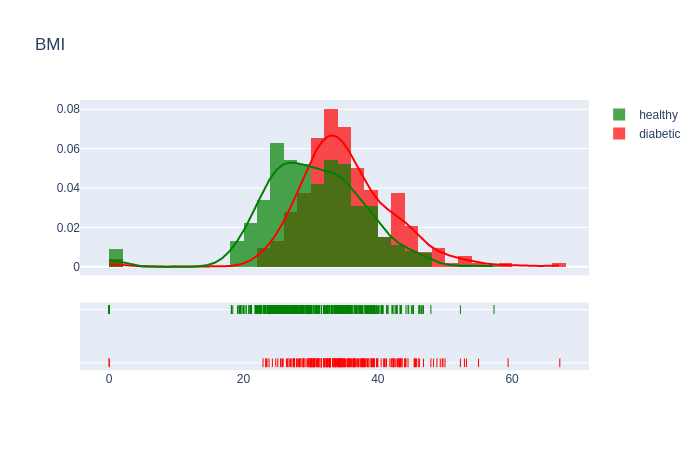
\includegraphics[width=1\textwidth]{10.png}
\caption{\label{fig:1} Subject distribution across Body Mass Index range.}
\end{figure}

\begin{figure}[ht]
\centering
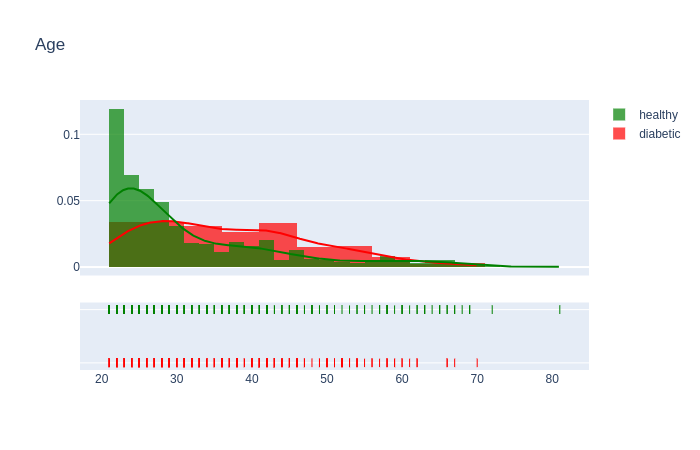
\includegraphics[width=1\textwidth]{11.png}
\caption{\label{fig:2} Subject distribution across age.}
\end{figure}

\begin{figure}[ht]
\centering
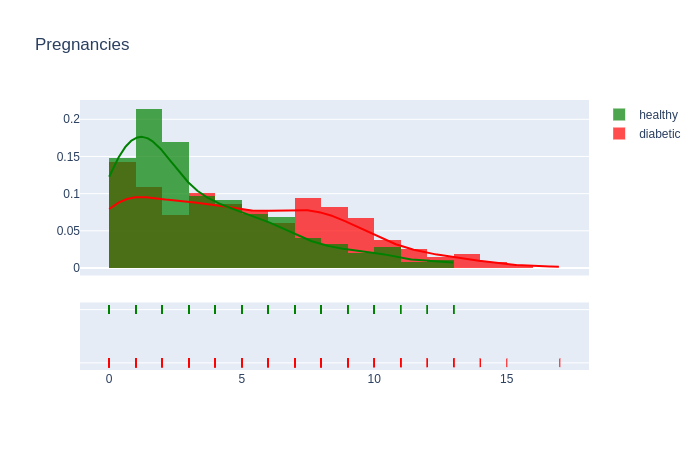
\includegraphics[width=1\textwidth]{12.png}
\caption{\label{fig:3} Subjects distribution via Pregnancies.}
\end{figure}

\begin{figure}[ht]
\centering
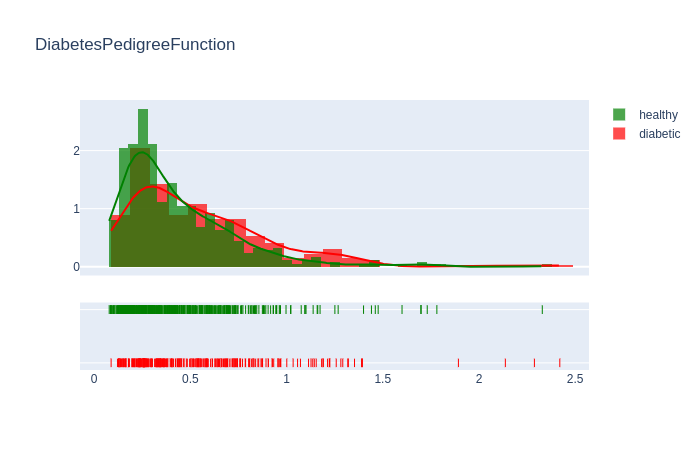
\includegraphics[width=1\textwidth]{13.png}
\caption{\label{fig:4} Subjects distribution via Diabetes Pedigree Function.}
\end{figure}

\begin{figure}[ht]
\centering
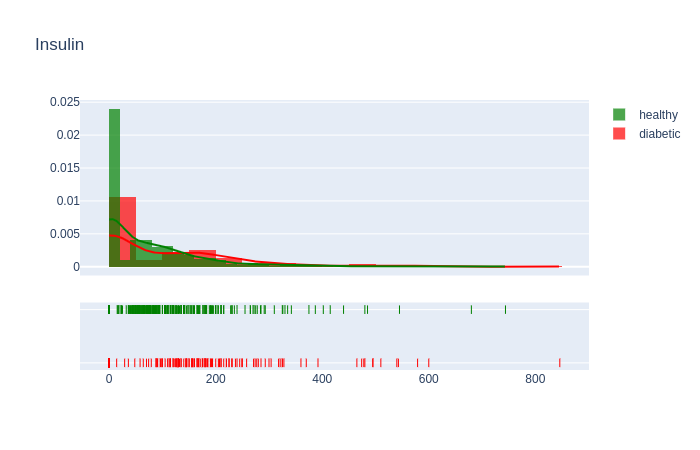
\includegraphics[width=1\textwidth]{14.png}
\caption{\label{fig:5} Subjects Insulin Distribution across ranges.}
\end{figure}

\begin{figure}[ht]
\centering
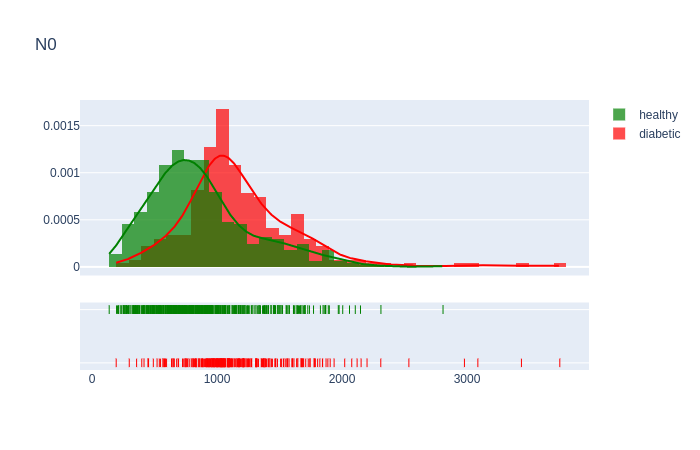
\includegraphics[width=1\textwidth]{15.png}
\caption{\label{fig:6} Plot of N0}
\end{figure}

\begin{figure}[ht]
\centering
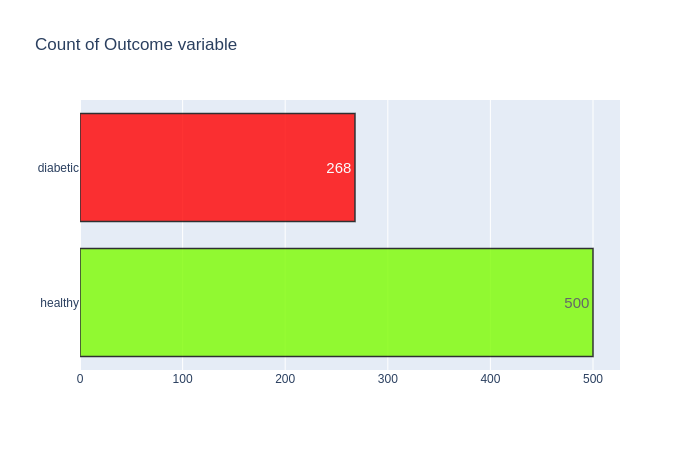
\includegraphics[width=1\textwidth]{1.png}
\caption{\label{fig:8} Diabetic v/s Healthy Subject Count.}
\end{figure}

\begin{figure}[ht]
\centering
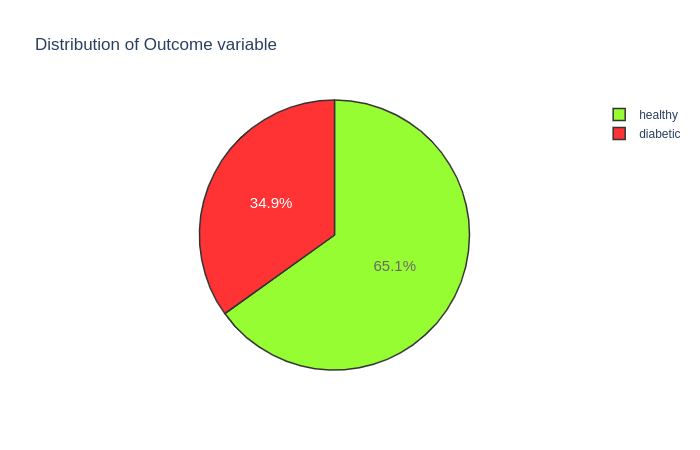
\includegraphics[width=1\textwidth]{2.png}
\caption{\label{fig:9} Diabetic v/s Healthy Subjects Percentage.}
\end{figure}

\begin{figure}[ht]
\centering
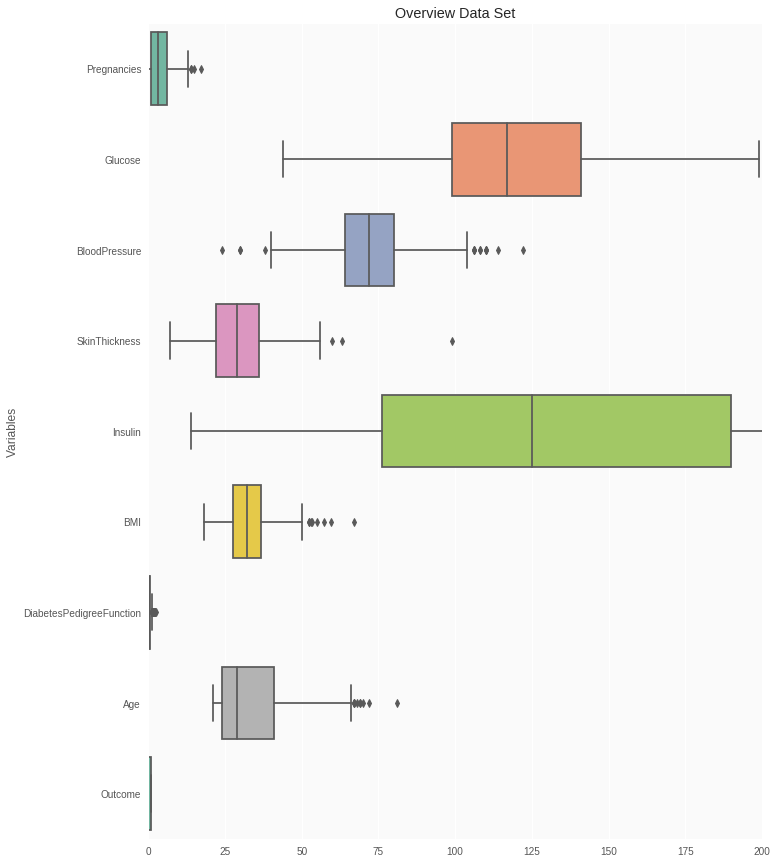
\includegraphics[width=1\textwidth]{3.png}
\caption{\label{fig:10} Boxplot for all attributes with outliers.}
\end{figure}

\begin{figure}[ht]
\centering
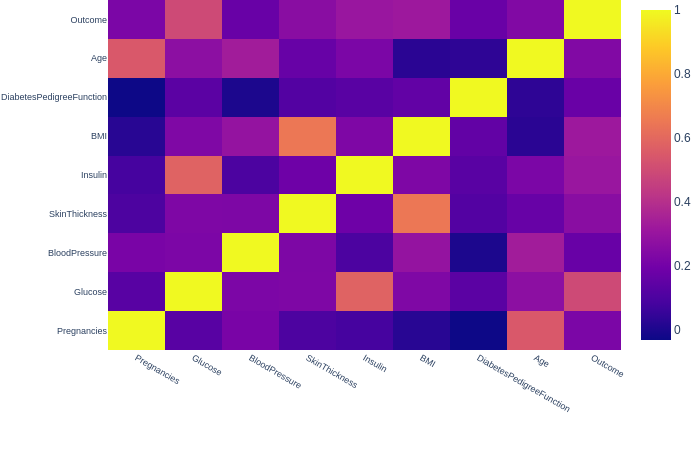
\includegraphics[width=1\textwidth]{4a.png}
\caption{\label{fig:11} Heatmap using Pearsons Correlation Coefficient.}
\end{figure}

\begin{figure}[ht]
\centering
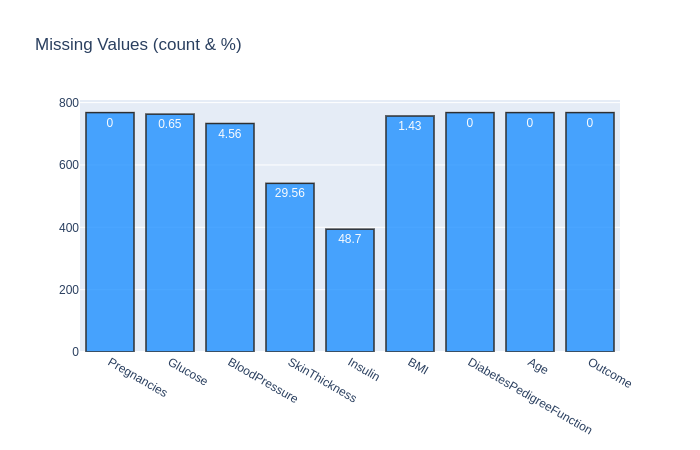
\includegraphics[width=1\textwidth]{4.png}
\caption{\label{fig:12} Number of missing values in count and percentage.}
\end{figure}

\begin{figure}[ht]
\centering
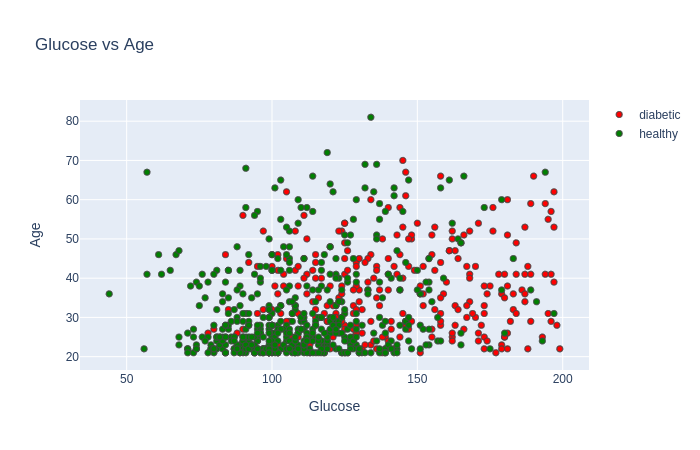
\includegraphics[width=1\textwidth]{5.png}
\caption{\label{fig:13} Glucose v/s Age scatterplot.}
\end{figure}

\begin{figure}[ht]
\centering
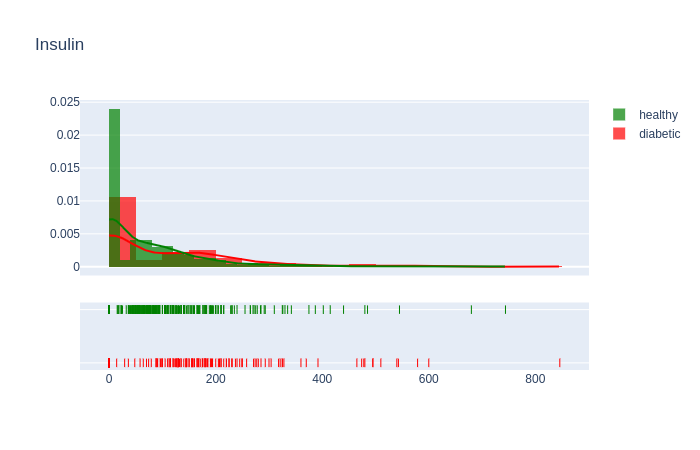
\includegraphics[width=1\textwidth]{6.png}
\caption{\label{fig:14} Subjects Insulin distributon.}
\end{figure}

\begin{figure}[ht]
\centering
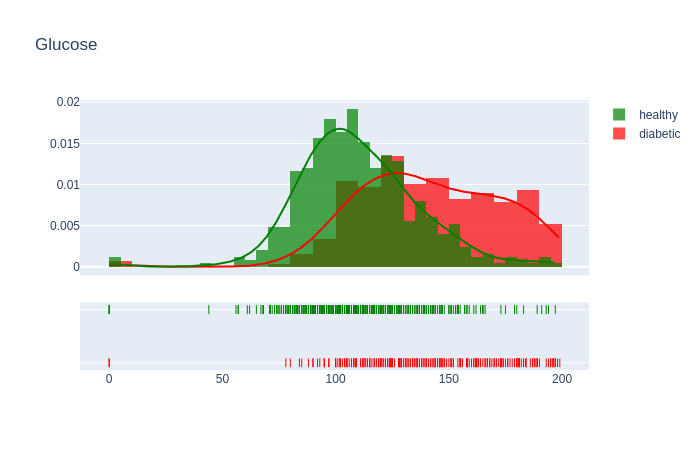
\includegraphics[width=1\textwidth]{7.png}
\caption{\label{fig:15} Subjects glucose distribution.}
\end{figure}

\begin{figure}[ht]
\centering
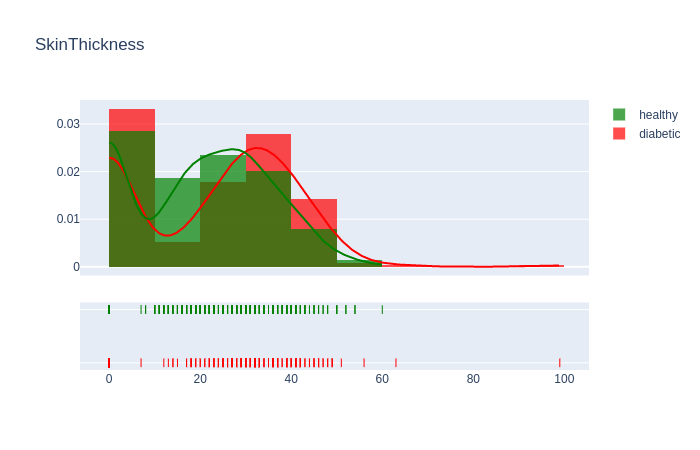
\includegraphics[width=1\textwidth]{8.png}
\caption{\label{fig:16} Skin Thickness distribution of subjects.}
\end{figure}

\begin{figure}[ht]
\centering
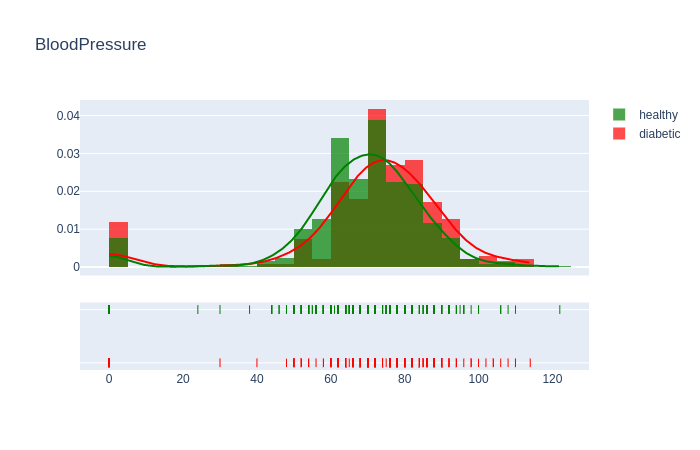
\includegraphics[width=1\textwidth]{9.png}
\caption{\label{fig:17} Blood Pressure distribution of subjects.}
\end{figure}

\begin{figure}[ht]
\centering
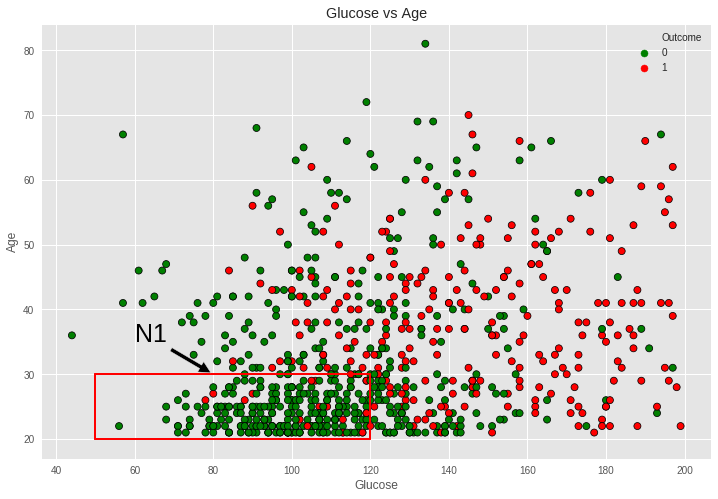
\includegraphics[width=1\textwidth]{download(1).png}
\caption{\label{fig:18} New feature N1.}
\end{figure}

\begin{figure}[ht]
\centering
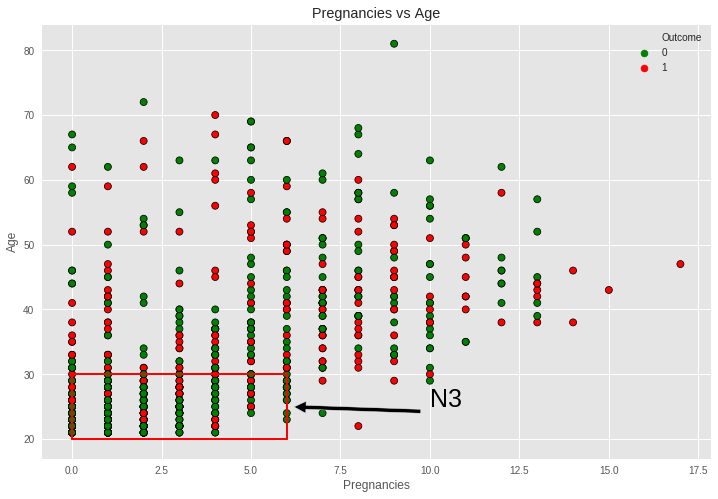
\includegraphics[width=1\textwidth]{download(2).png}
\caption{\label{fig:19} New feature N3.}
\end{figure}

\begin{figure}[ht]
\centering
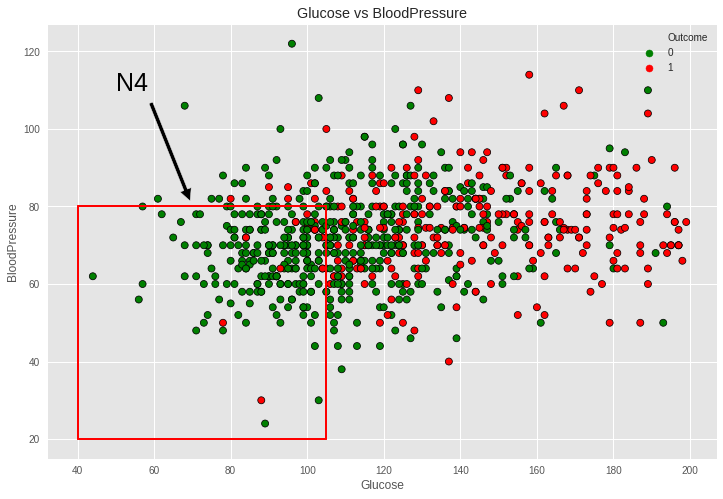
\includegraphics[width=1\textwidth]{download(3).png}
\caption{\label{fig:20}  New feature N4.}
\end{figure}

\begin{figure}[ht]
\centering
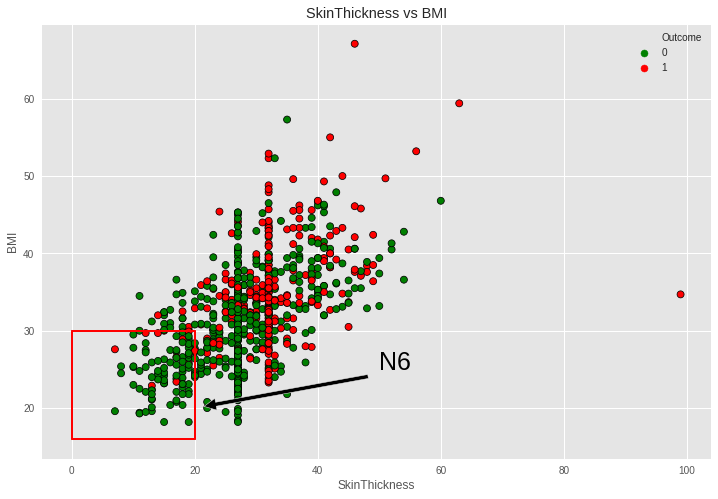
\includegraphics[width=1\textwidth]{download(4).png}
\caption{\label{fig:21}  New feature N6.}
\end{figure}

\begin{figure}[ht]
\centering
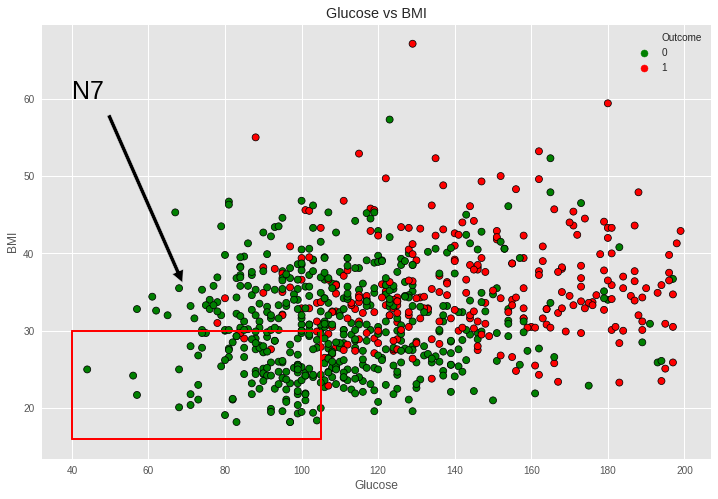
\includegraphics[width=1\textwidth]{download(5).png}
\caption{\label{fig:22}  New feature N7.}
\end{figure}

\begin{figure}[ht]
\centering
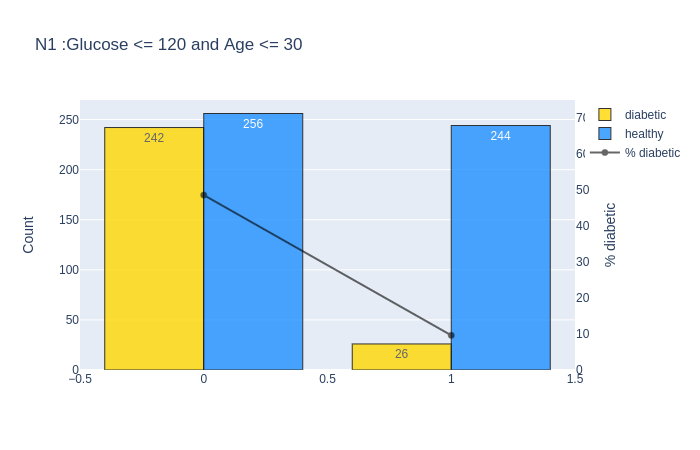
\includegraphics[width=1\textwidth]{newplot(13).png}
\caption{\label{fig:23} N1 barplot for diabetic and healthy population.}
\end{figure}

\begin{figure}[ht]
\centering
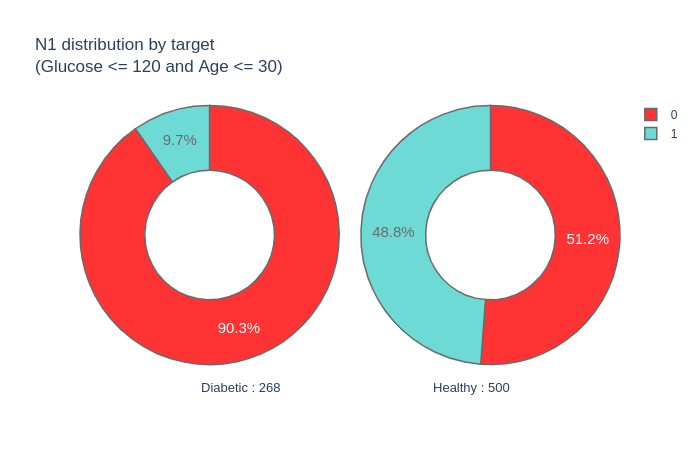
\includegraphics[width=1\textwidth]{newplot(14).png}
\caption{\label{fig:24} N1 distribution in percentage.}
\end{figure}

\begin{figure}[ht]
\centering
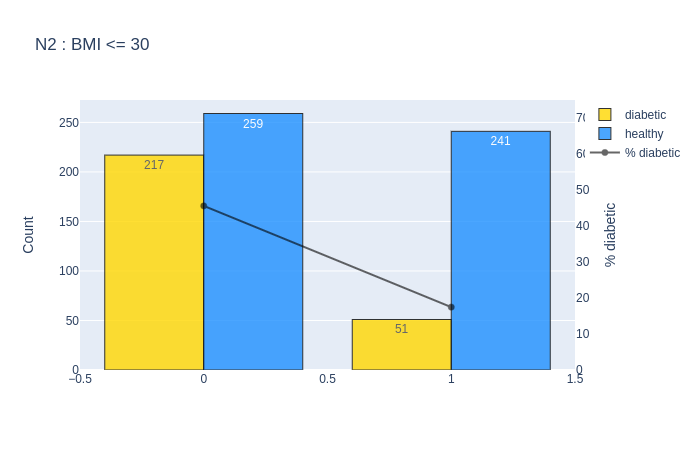
\includegraphics[width=1\textwidth]{newplot(15).png}
\caption{\label{fig:25} N2 barplot for diabetic and healthy population.}
\end{figure}

\begin{figure}[ht]
\centering
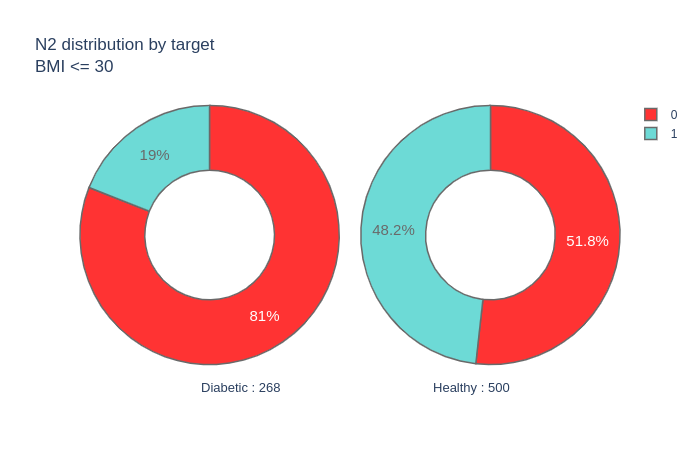
\includegraphics[width=1\textwidth]{newplot(16).png}
\caption{\label{fig:26} N2 distribution in percentage.}
\end{figure}

\begin{figure}[ht]
\centering
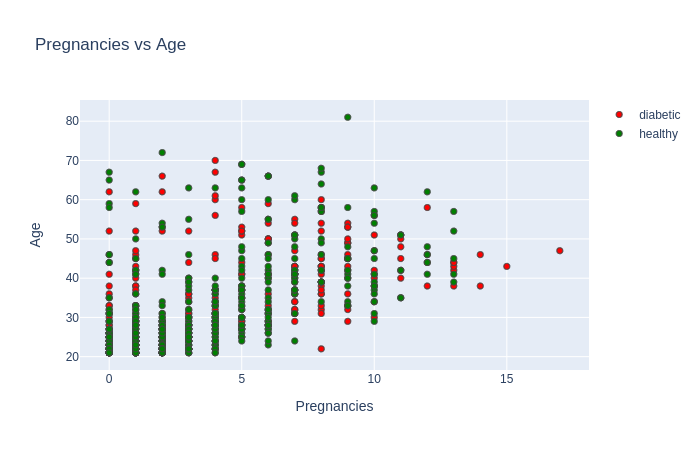
\includegraphics[width=1\textwidth]{newplot(17).png}
\caption{\label{fig:27} Pregnancies v/s age scatterplot.}
\end{figure}

\begin{figure}[ht]
\centering
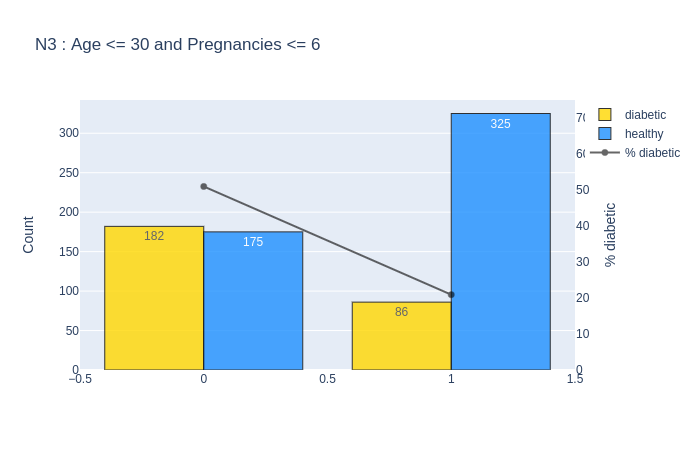
\includegraphics[width=1\textwidth]{newplot(18).png}
\caption{\label{fig:28} N3 barplot for diabetic and healthy population.}
\end{figure}

\begin{figure}[ht]
\centering
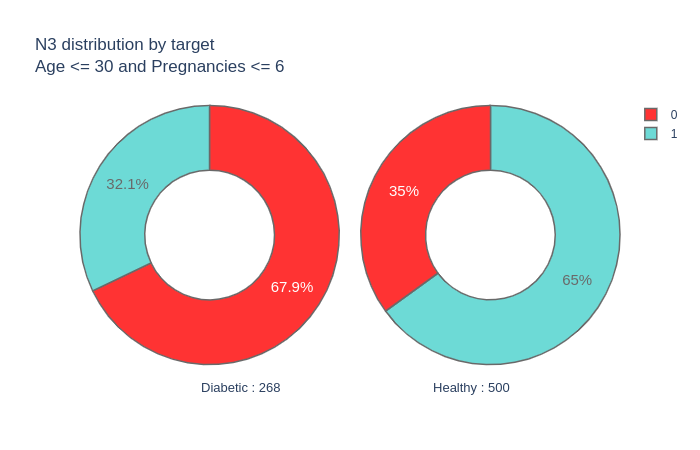
\includegraphics[width=1\textwidth]{newplot(19).png}
\caption{\label{fig:29} N3 distribution in percentage.}
\end{figure}

\begin{figure}[ht]
\centering
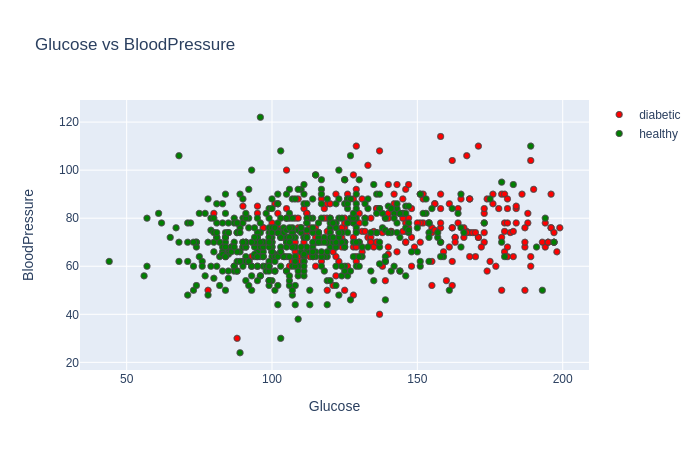
\includegraphics[width=1\textwidth]{newplot(20).png}
\caption{\label{fig:30} Glucose v/s Blood Pressure scatterplot.}
\end{figure}

\begin{figure}[ht]
\centering
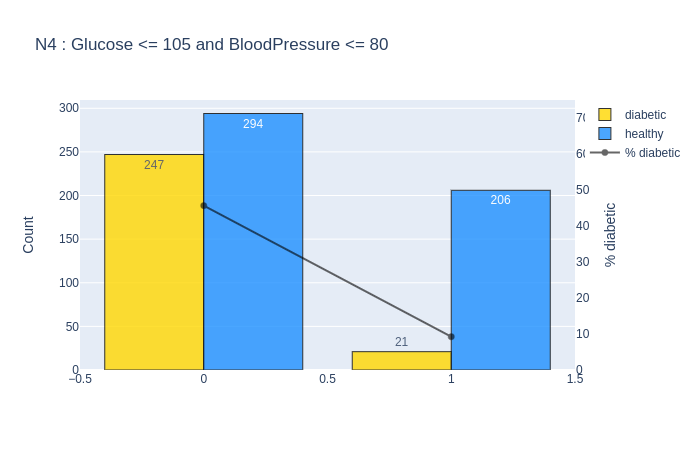
\includegraphics[width=1\textwidth]{newplot(21).png}
\caption{\label{fig:31} N4 barplot for diabetic and healthy population.}
\end{figure}

\begin{figure}[ht]
\centering
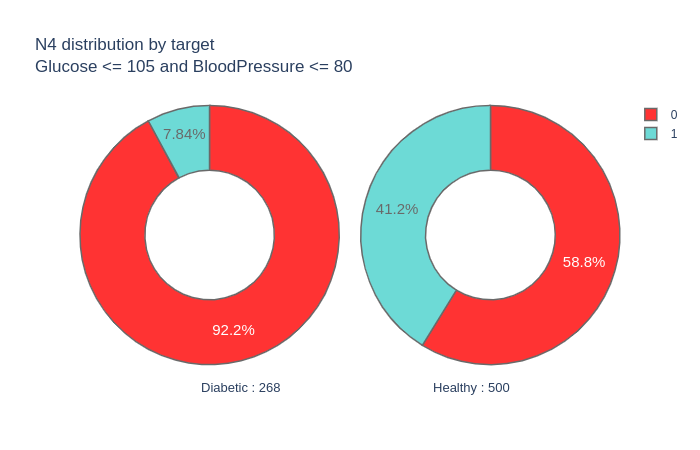
\includegraphics[width=1\textwidth]{newplot(22).png}
\caption{\label{fig:32} N4 distribution by target.}
\end{figure}

\begin{figure}[ht]
\centering
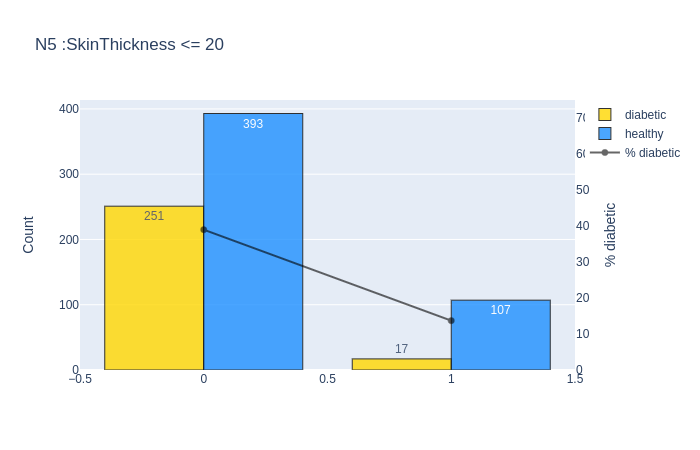
\includegraphics[width=1\textwidth]{newplot(23).png}
\caption{\label{fig:33} N5 barplot for diabetic and healthy population.}
\end{figure}

\begin{figure}[ht]
\centering
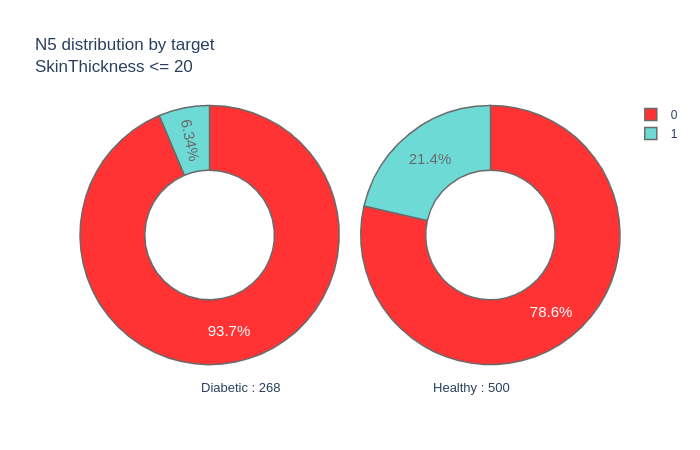
\includegraphics[width=1\textwidth]{newplot(24).png}
\caption{\label{fig:34} N5 distribution by target.}
\end{figure}

\begin{figure}[ht]
\centering
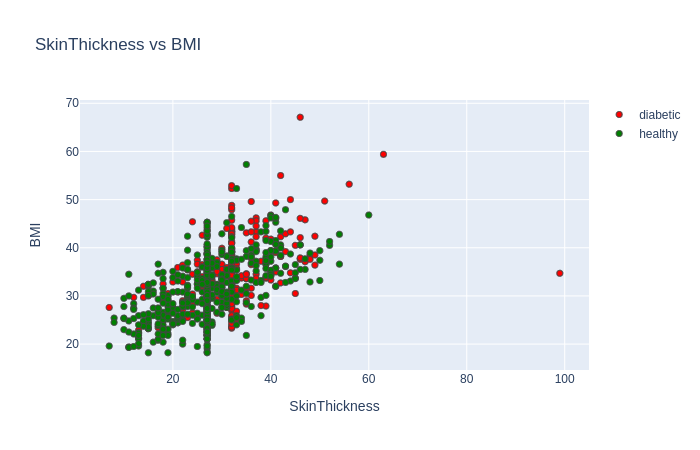
\includegraphics[width=1\textwidth]{newplot(25).png}
\caption{\label{fig:35} Skin Thickness v/s BMI scatterplot.}
\end{figure}

\begin{figure}[ht]
\centering
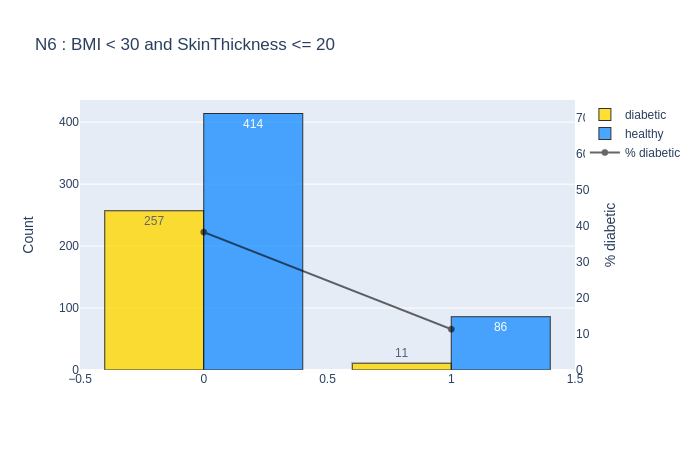
\includegraphics[width=1\textwidth]{newplot(26).png}
\caption{\label{fig:36} N6 barplot for diabetic and healthy population.}
\end{figure}

\begin{figure}[ht]
\centering
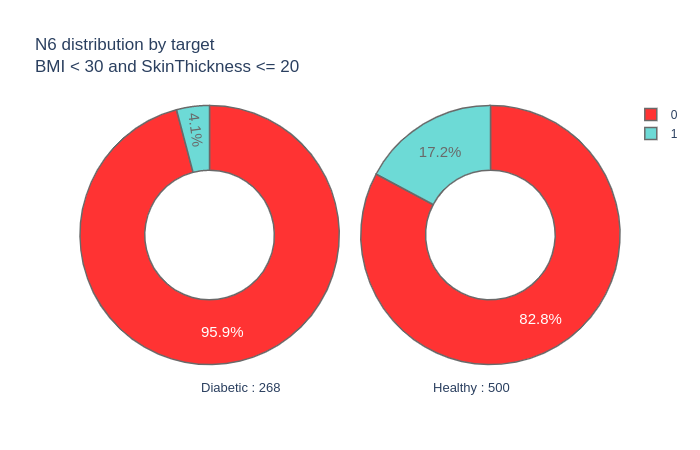
\includegraphics[width=1\textwidth]{newplot(27).png}
\caption{\label{fig:37} N6 distribution by target.}
\end{figure}

\begin{figure}[ht]
\centering
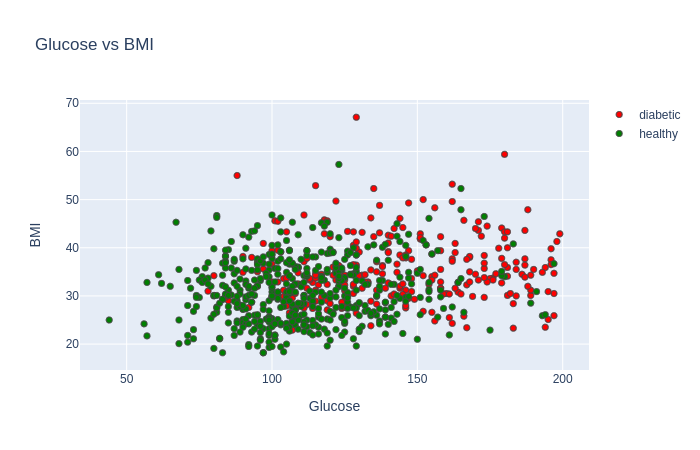
\includegraphics[width=1\textwidth]{newplot(28).png}
\caption{\label{fig:38} Glucose v/s Body Mass Index scatterplot.}
\end{figure}

\begin{figure}[ht]
\centering
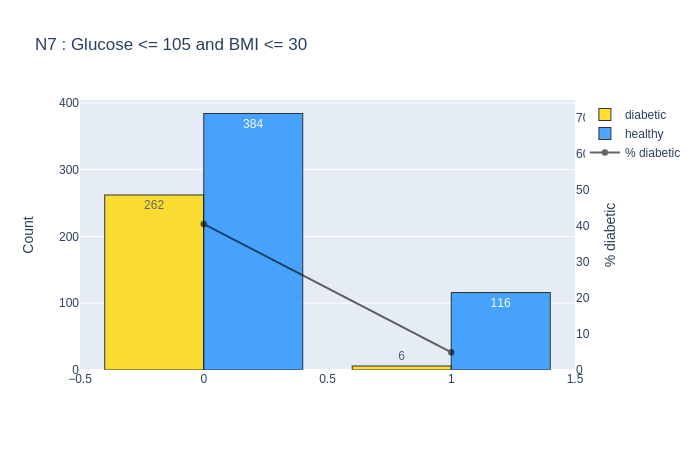
\includegraphics[width=1\textwidth]{newplot(29).png}
\caption{\label{fig:39} N7 barplot for diabetic and healthy population.}
\end{figure}

\begin{figure}[ht]
\centering
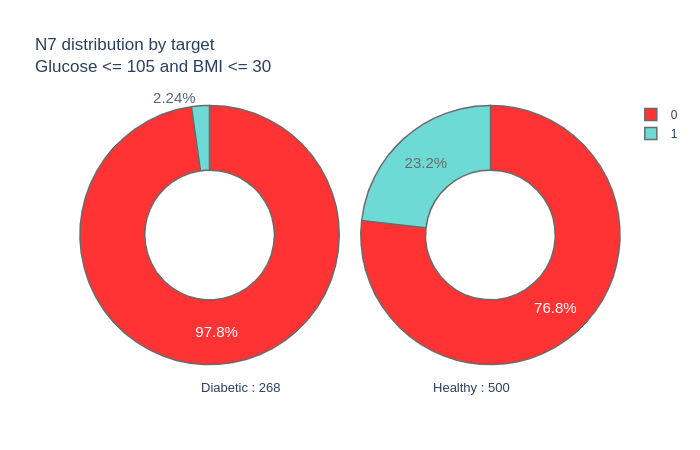
\includegraphics[width=1\textwidth]{newplot(30).png}
\caption{\label{fig:40} N7 distribution by target.}
\end{figure}

\begin{figure}[ht]
\centering
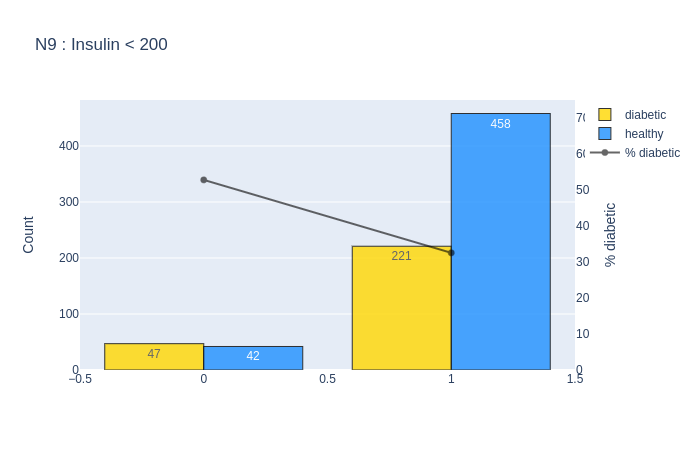
\includegraphics[width=1\textwidth]{newplot(32).png}
\caption{\label{fig:41} N9 barplot for diabetic and healthy population.}
\end{figure}

\begin{figure}[ht]
\centering
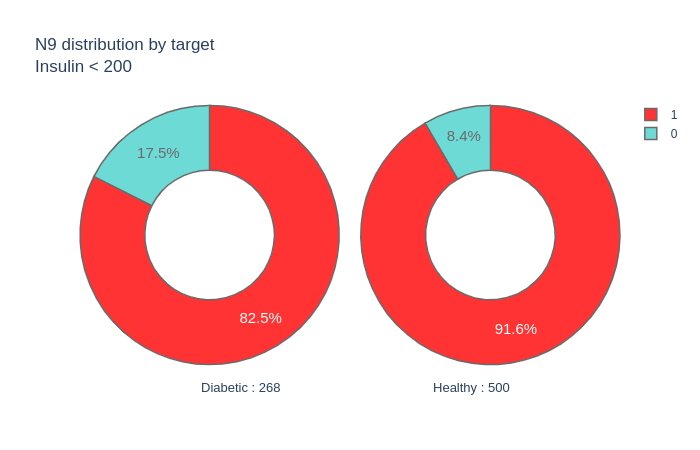
\includegraphics[width=1\textwidth]{newplot(33).png}
\caption{\label{fig:42} N9 distribution by target.}
\end{figure}

\begin{figure}[ht]
\centering
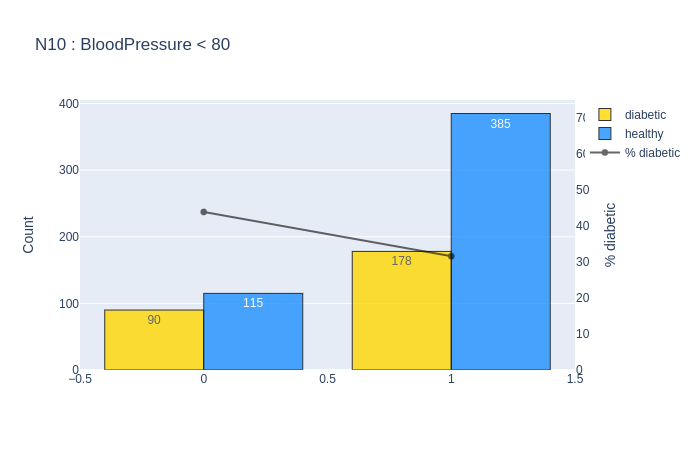
\includegraphics[width=1\textwidth]{newplot(34).png}
\caption{\label{fig:43} N10 barplot for diabetic and healthy population.}
\end{figure}

\begin{figure}[ht]
\centering
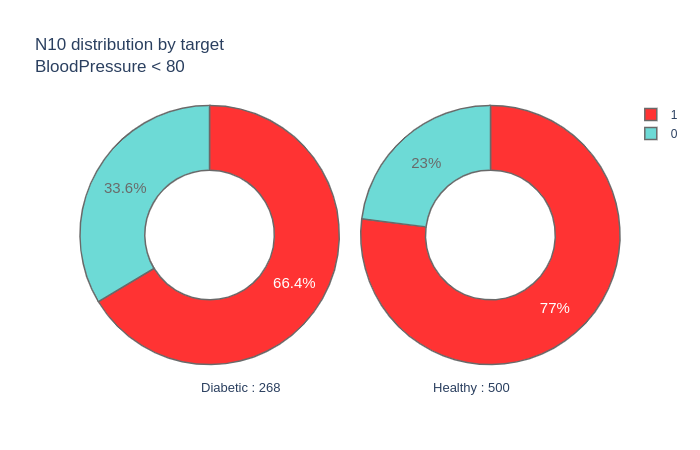
\includegraphics[width=1\textwidth]{newplot(35).png}
\caption{\label{fig:44} N10 distribution by target.}
\end{figure}

\begin{figure}[ht]
\centering
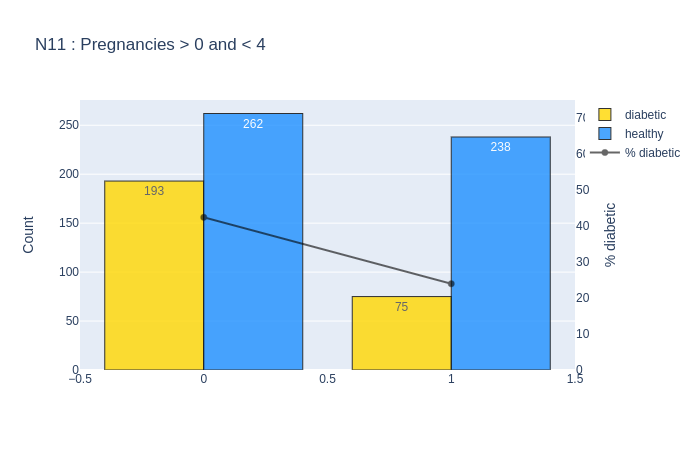
\includegraphics[width=1\textwidth]{newplot(37).png}
\caption{\label{fig:45} N11 barplot for diabetic and healthy population.}
\end{figure}

\begin{figure}[ht]
\centering
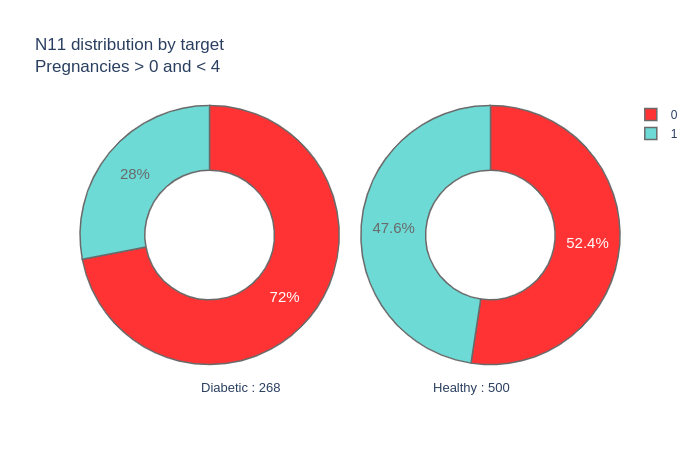
\includegraphics[width=1\textwidth]{newplot(38).png}
\caption{\label{fig:46} N11 distribution by target.}
\end{figure}

\begin{figure}[ht]
\centering
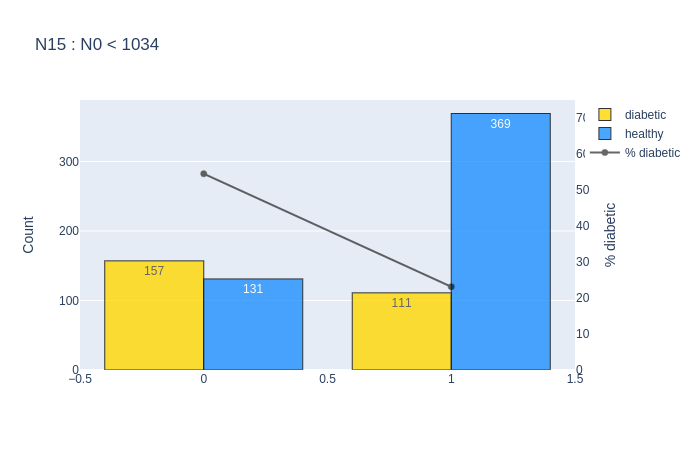
\includegraphics[width=1\textwidth]{newplot(40).png}
\caption{\label{fig:47} N15 barplot for diabetic and healthy population.}
\end{figure}

\begin{figure}[ht]
\centering
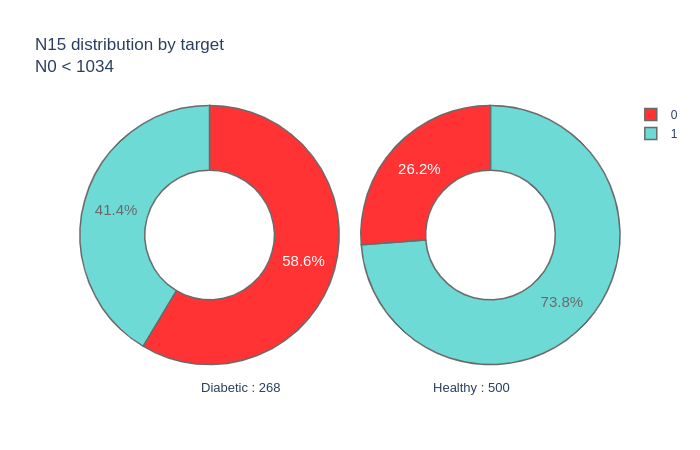
\includegraphics[width=1\textwidth]{newplot(41).png}
\caption{\label{fig:48} N15 distribution by target.}
\end{figure}

\begin{figure}[ht]
\centering
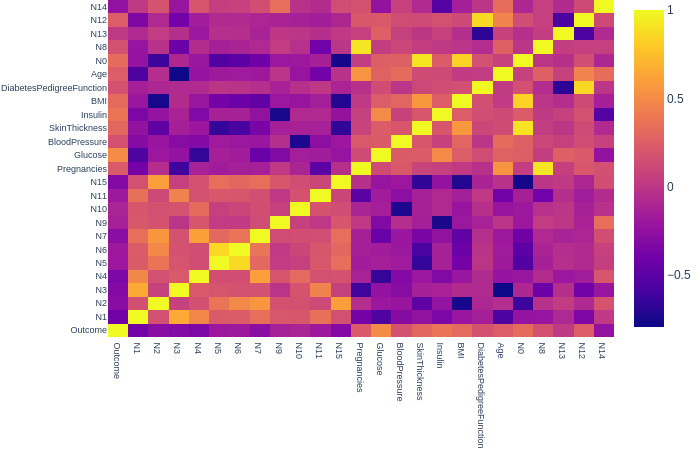
\includegraphics[width=1\textwidth]{newplot(42).png}
\caption{\label{fig:49} Extended heatmap with new features combined.}
\end{figure}

\clearpage
\newpage
\section{Conclusion}

\clearpage
\newpage
\nocite{*}
\bibliographystyle{plain}
\bibliography{bib}
\end{document}
